\chapter{System Implementation} \label{chap:implementation}

This chapter describes the implementation aspects of our Virtual and Distributed HSM. Each section analyses a specific protocol, starting with the Distributed Key Generation, then the Threshold Signatures, and ending with the Threshold Symmetric Encryption. Each provides a more in-depth view of its features, implementation, and integration with COBRA.

\section{Distributed Key Generation} \label{sec:distributedkeygen}

A Distributed Key Generation (DKG) protocol is a fundamental building block of symmetric and asymmetric threshold cryptography. It solves the problems of single point of failure and key escrow, when there is a trusted authority that holds a secret, by using a complete distribution of shares of the secret among a set of servers, being the servers who will jointly agree on a secret, in contrast to the original secret sharing schemes \cite{shamir}, which required a leader to generate a secret and distribute its shares among participating parties.

The distributed polynomial generation protocol of COBRA \cite{cobra} served as the foundation for implementing our distributed key generation. This protocol does not require a designated leader to generate and distribute the shares of the secret. Instead, the protocol allows a group of servers to collectively create a random polynomial \textit{P} of degree \textit{t} with an encoded random point $(x, y)$ in a distributed manner. 

Each server in the group independently generates a random polynomial and distributes its shares to the other servers in the group. Subsequently, the servers run a Byzantine consensus algorithm to ensure that honest servers select the same set of $t + 1$ of these random polynomials. The selected polynomials are then summed, resulting in the shares of a polynomial \textit{P}. The protocol ensures that at least $t + 1$ correct servers obtain a valid share of the secret encoded in polynomial \textit{P}, and the other correct servers will detect invalid shares. This consensus process allows the servers to collectively agree on the shares of the polynomial \textit{P} without relying on a designated leader. The secret encoded in this random distributed polynomial can hence be used as a cryptographic key, remaining secret until a client decides to reconstruct it, which, in the case of our HSM, they never will as it is an operation that is not available. Nevertheless, since its shares are distributed throughout the servers, it can be used ``as is" for threshold signatures and encryption, i.e., without requiring additional client interaction.

To perform signatures with a specific algorithm, the required keys to issue the signature must follow a set of configurations, i.e., values that allow the construction of a distinct elliptic curve. The same signature algorithm can issue signatures using different elliptic curves, while others require a particular one. As we intended the system to be able to perform valid and compatible signatures for the Bitcoin and Ethereum blockchains, we would need to implement at least two different elliptic curve configurations. However, the previous protocol, and COBRA as a whole, were only compatible with the \texttt{secp256r1} elliptic curve, and the system was not prepared to be extended in this regard.

To work around this problem of being limited to a single elliptic curve, we had to guarantee that the functionalities that COBRA depends on would not be affected. With that in mind, we decided on the following solution:
\begin{itemize}
    \item When starting up the HSM replicas, for each desired elliptic curve, we initialize an instance of the \texttt{CobraConfidentialityScheme} class since this is the main class from where these configurations are called and obtained;
    
    \item The created instances are then registered in a map under the \texttt{DistributedPolynomial} class, which is the main class for generating the distributed polynomials. Each stored instance in the map is associated with the name of the elliptic curve it implements, acting as the entry key. We will be referring to it as \textit{confidentialitySchemeId};
    
    \item When a request is received, the \textit{confidentialitySchemeId} associated with the processed operation is propagated by the HSM servers to COBRA, so the correct scheme is used when performing the protocol;

    \item When executing the protocol, for all the servers to be in the same state and to avoid conflicts when receiving both different requests and signatures, we added the \textit{confidentialSchemeId} as a new field to the \texttt{PolynomialMessage} class, responsible for the messages that are changed between the servers during the distributed polynomial generation protocol. When decoding the received messages, it would enable each server to use the proper confidentiality scheme instance, obtainable from the initial map.
\end{itemize}%fazer uma figura com os passos que acontecem quando é recebido um pedido para gerar uma nova have

This way, the system will not be limited to only one or two elliptic curves but to an arbitrary number of different ones, requiring only the configuration of the desired curves in the \texttt{HsmServer} file, although these also need to be compatible with the available algorithms.

At the moment, besides the native one that was previously installed, \texttt{secp256r1}, the system supports two new elliptic curves, \texttt{secp256k1} and \texttt{BLS12-381}, enabling the creation of cryptographic keys compatible with the Bitcoin and Ethereum blockchains, respectively, since cryptocurrency wallets are a use case of our project. These two last curves allow for the generation of keys compatible with two different signature schemes, Schnorr and BLS, respectively, which will be covered in the next section. 

The DKG protocol enables the creation of a secret or a private key depending on the final purpose. Therefore, when generating a private key, the corresponding public key is created differently depending on the signature scheme. In the protocol implemented for the Schnorr signature, the public key corresponds to the commitment of the generated private key, while for the BLS scheme, we use a third-party library to create a compatible public key. Regarding symmetric keys, since our encryption algorithm is not a traditional protocol, it does not require a specific type of symmetric key, so for this case, we simply generate a secret key using the DKG protocol, which, in our case, will act as a symmetric key in a centralized encryption algorithm. 

\section{Threshold Signatures} \label{sec:thresholdsignatures}

With the help of a threshold signature scheme (TSS), multiple parties can jointly calculate a signature without sharing any details about the private key. Schnorr and BLS signatures were chosen to be implemented since they are non-interactive and present advantages related to simplicity and performance. They were recently implemented in the most known blockchains, Bitcoin and Ethereum, respectively, eventually leading to smaller blockchains following their steps.

To implement the Schnorr signature \cite{schnorrnotes} in a threshold manner we utilized a version of the protocol already implemented in the SIRE project \cite{siregithub}, which was inspired by the ROAST proposal \cite{frost3}, and for the BLS signature \cite{blsdraft} we used the RELIC library \cite{relicgithub} which already provides all the necessary functions to sign, combine, and verify the signatures and key pairs. Both schemes allow the aggregation of partial signatures into a final signature, and the BLS signatures enable the grouping of private/public keys into a single key pair. Therefore, each server starts by producing its share of the signature, i.e., a partial signature and public key, and then, the client is responsible for combining them into the final signature and public key.

As previously stated, the high-level algorithm of both signatures corresponds only to a two-round client-server communication. During the first, the client submits the request with the necessary information to issue the signature, specifically, a hash of the message to be signed, the index ID of the private key to be used, and the signature scheme. In the second round, the servers respond with a partial signature constructed using the private key share each of them possesses. After receiving the required number of partial results, the client verifies their integrity and combines them into the final signature.

Regarding the Schnorr signature scheme, the algorithm performed by each replica to generate the partial signature is very similar to the regular centralized version. After the replicas conclude the distributed key generation protocol, due to the need for a random value $k$, they start by computing a hash $H$ of the data to be signed $M$ with the public key of the generated value $r$, $e=H(M || r)$, where $||$ denotes concatenation. The partial signature is completed by computing $s_i=k_i + e \cdot sk_i$, where $sk_i$ corresponds to the private key share associated with the index ID provided by the client. When the partial signatures are received, the client verifies them using the commitments of both the private key and the random key value, which were sent with the partial results, and then combines them into the final signature using the Lagrange Interpolation with the valid partial signatures. Due to the need for a new random key value for every Schnorr signature to avoid a possible key leakage from reusing this nonce, the key generation and the Schnorr signature operations are the only ones that require the replicas to communicate among themselves since we need to invoke the DKG protocol again to generate this random value.

Concerning the BLS signature scheme, we use the RELIC library~\cite{relicgithub}, a modern research-oriented cryptographic toolkit emphasizing efficiency and flexibility implemented in the C language, to compute the signatures. An exciting feature of this scheme is that the signatures and public keys can act as final or partial values, depending on our objective. Just like in threshold Schnorr signatures, the only difference when calculating the signature to become threshold is that where the private key was used, we now replace it with the private key share instead, $s_i=H(M) \cdot sk_i$. We use this library to calculate the public key share (corresponding to the private key share stored by each replica), issue the signatures using the private key share, verify the signatures' validity, and perform the Lagrange Interpolation to build the final signature and public key.


\section{Threshold Symmetric Encryption} \label{sec:thresholdencryption}
% talvez fazer uma figurinha com o funcionamento do algoritmo, tipo o client envia um pedido, com o commit da data, e cada servidor envia a sua contribution para o client, este constroi o ciphertext, e mais tarde envia o commit de volta para o servidor para realizar a decryption, que corresponds aos mesmos passos da encryption.

To achieve a practical and efficient threshold symmetric encryption, we implemented the most distinguished proposal in this field, discussed in Section \ref{subsec:threshold-encryption}, named \textit{Distributed Symmetric-key Encryption} (DiSE) \cite{dise}. The idea of the protocol consists of a generic construction of threshold authenticated encryption based on any distributed pseudorandom function (DPRF), where each server produces a partial result that the client will then combine to produce the final ciphertext, or the original message when performing the decryption. 

A technical view of the implemented protocol is illustrated in Figure \ref{fig:5.3.dise-protocol}. To adapt this algorithm to our system, we utilize our DKG protocol to generate and distribute the secret key shares among the replicas, and as the authors did in their implementation, we use \texttt{SHA3-256} as a commitment scheme and the AES algorithm as the pseudorandom number generator. Specifically, as described in the API specification of the previous chapter, the clients will first generate a secret key using the DKG (which we consider to be our symmetric key), so later they can use the pre-generated secret key to perform an encryption or decryption by providing the \texttt{indexId} associated to the key during its creation.

\begin{figure}[h]
    \begin{center}
        \resizebox{80mm}{!}{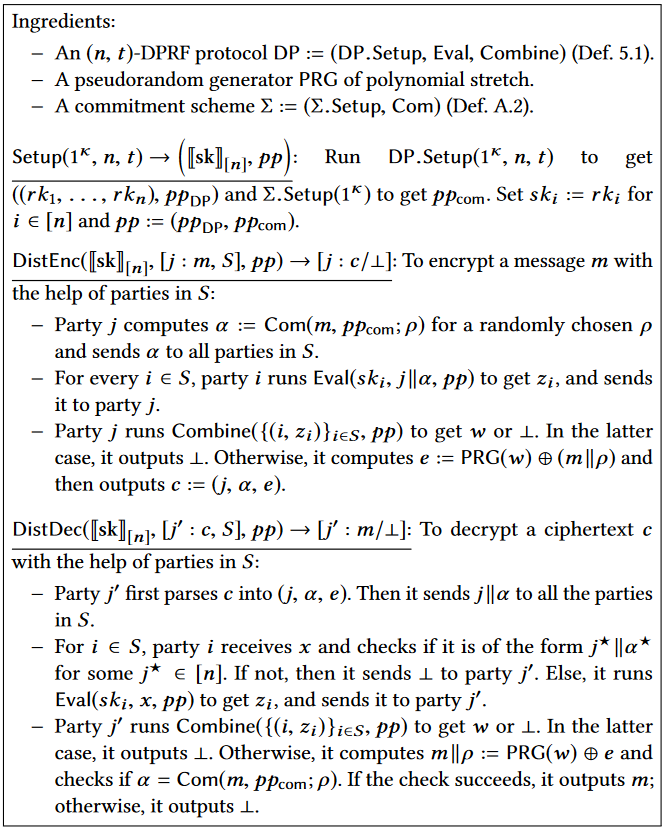
\includegraphics[]{5.3.dise-protocol}}
    \end{center}
    \caption{The implemented DiSE protocol \cite{dise}.}
    \label{fig:5.3.dise-protocol}
\end{figure}

The DPRF is the algorithm's most crucial component. Its responsibility is to generate partial results deterministically. Being deterministic is the key factor for making possible a later decryption of a ciphertext previously encrypted by this same protocol.

The applied DPRF was inspired by the algorithm depicted in Figure 6 of the DiSE paper~\cite{dise}, corresponding to a privately verifiable version, secure under the Decisional Diffie-Hellman assumption~\cite{ddh}, that requires only two communication rounds to conclude its protocol. It was adapted by Robin Vassantlal, author of COBRA, joining it to a previous version of a DPRF that he had implemented when developing his project, adjusting the protocol to support the usage of elliptic curves. Afterward, we extended this implementation to use the Distributed Key Generation described above in its setup phase, allowing each replica to agree on a polynomial and obtain their shares in a distributed manner. The final version of the DPRF algorithm contains the following steps:
\begin{itemize}
    \item \textbf{Init:} Performs the DKG protocol, distributing the secret key shares among the servers $(sk_1, ..., sk_n)$ and sets the constant parameters, i.e., the elliptic curve configuration, where $g$ corresponds to the curve generator which is the $(x, y)$ point in the curve, and $rho$, corresponding to the curve's prime order. In the end, each server's private and public parameters ($pp$) are obtained. The former contains the secret key share, which never leaves the corresponding server, and the latter holds the commitment of the key share ($com_{sk_i}$), being the only information sent to the client;

    \item \textbf{Contribute}$(sk_i, x, pp)$: Computes $w = g \cdot x$ and $h_i = w \cdot sk_i$. Picks $v_i \leftarrow \mathbb{Z}_\rho$ and sets $t_i = w \cdot v_i$. After calculating all these variables, computes the final hash $c_i = \mathcal{H}(h_i, w, com_{sk_i}, g, t_i)$ and $u_i = v_i - c_i \cdot sk_i$. Resulting in the output $z_i = (h_i, c_i, u_i)$, which corresponds to the partial result;

    \item \textbf{Evaluate}$({(i, z_i)}_{i \in S}, pp)$: If the number of received contributions $S$ is less than the required $t$, return $\perp$. Otherwise, parse $z_i$ as $((w, h_i), (c_i, u_i))$ for $i \in S$. Compute $t_i = w \cdot u_i + h_i \cdot c_i$ and check if $c_i = \mathcal{H}'(h_i, w, com_{sk_i}, g, t_i)$. If check fails for any $i \in S$, return $\perp$, else return $\sum_{i \in S}h_i \cdot \lambda_{0, i, S}$, where $\lambda_{0, i, S}$ correspond to the Lagrange coefficients.
\end{itemize}

A key characteristic of this algorithm is that the clients send to the servers only a commitment of the data they want to encrypt. This way, the size of the data will not influence the system's performance. The commit corresponds to the hash of the data to encrypt together with a random value, allowing the initial data to remain secret to the servers throughout the entire process.

In the end, the resulting ciphertext includes the identifier of the \textit{encryptor}, i.e., the client's identifier who aggregated the partial results into the final ciphertext, the committed data, and the actual encryption. Later, if not tampered with, these additional properties will allow the protocol to retrieve the corresponding initial message.

\section{Final Remarks} \label{sec:impl-final-remarks}

In this chapter, we detailed the implementation particularities of each main protocol. We demonstrated how these algorithms achieved the previously referred properties of confidentiality, integrity, and availability by explaining each in-depth. We started with the Distributed Key Generation protocol, where, besides providing details of the algorithm, we clarified how we resolved the problem of expanding the protocol to allow the usage of any elliptic curves. Then, we elaborated a simplified version of the algorithms employed for the threshold signatures, namely, Schnorr and BLS signature schemes. Finally, we introduced a more technical description of the threshold symmetric encryption protocol utilized, DiSE. Specifically, we defined the chosen DPRF protocol and noted all the changes to adapt it to our needs. 

%\LIMPA